\textit{Средства разработки}. В качестве средства разработки применяется интегрированная среда Microsoft Visual Studio 2010. Эта среда разработки поддерживает компонентную технологию, позволяет легко создавать собственные компоненты и интегрироваться с внешними модулями ПО и офисными пакетами.

\textit{Требования к аппаратному и программному обеспечению}. Для нормального функционирования программы необходимы следующие программные и технические средства:
\begin{itemize}
  \item Intel-совместимый процессор с тактовой частотой не менее 1 ГГц;
  \item объём оперативной памяти~--- 1 ГБ и более;
  \item свободное место на жёстком диске~--- 100 МБ и более;
  \item операционная система~--- Windows 7 и выше;
  \item предустановленная среда выполнения .NET Framework Client Profile версии не ниже 4.0;
  \item предустановленный пакет визуализации Graphviz версии не ниже 2.28;
  \item предустановленный офисный пакет Microsoft Office версии не ниже 14 (Office 2010).
\end{itemize}

\textit{Условия применения программы.} Разработанная программа решает научно-исследовательскую и прикладную задачи. Программа распространяется свободно и без каких-либо ограничений и гарантий.

\subsection{Программный модуль CSBusinessGraph}

\subsubsection*{Назначение программы}

Разработанная программа предназначена для проведения вычислительного эксперимента по сетевому анализу проектов в условиях нечёткой неопределённости, цель которого заключалась в апробации описанных в~главе~\ref{chapter2} двухточечных вычислений и сравнении их результатов с результатами $\alpha$-уровневых вычислений.

\subsubsection*{Интерфейс пользователя}
Программа имеет интуитивно понятный интерфейс, представленный на рисунке~\ref{fig:app-main}. На нижней панели расположены элементы управления представлением~--- кнопки и ползунок, позволяющие изменять масштаб. Для создания нового проекта необходимо выбрать пункт меню <<File~--- New Project>> (Файл~--- Новый проект). Также возможна загрузка ранее созданного проекта для редактирования. Для этого необходимо выбрать пункт меню <<File~--- Open Existing Project>> (Файл~--- Открыть существующий проект), после чего будет показан диалог открытия файла 
\begin{figure}[h!]
  \centering
  {
    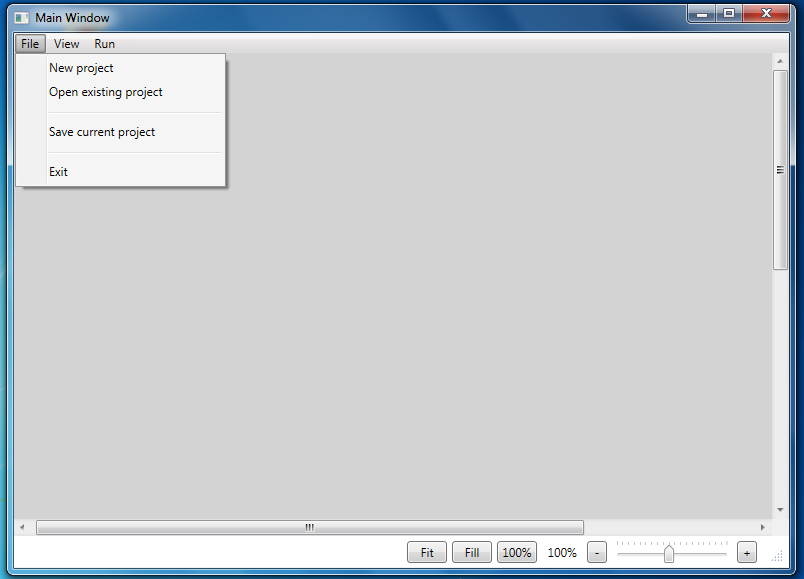
\includegraphics[width=0.85\textwidth]{app-main.png}
  }
  \caption{Главное окно приложения на старте}
  \label{fig:app-main}
\end{figure}

Вначале создаются операции путём вызова контекстного меню (рисунок~\ref{fig:app-sample-graph}) и нажатия на опцию <<Create Node>> (Создать узел). При этом появляется окно для ввода и редактирования данных операции, представленное на рисунке~\ref{fig:app-edit-window}. Это~же окно можно вызвать, выделив вершину графа и~нажав пункт меню <<View>> (Просмотр). Создание дуги выполняется с помощью механизма <<drag-and-drop>>: левая кнопка мыши нажимается в одной из двух точек узла, называемых точками сопряжения, и отпускается после перетаскивания курсора на вершине, в которую должна входить дуга. 

\begin{figure}[b!]
  \centering
  {
    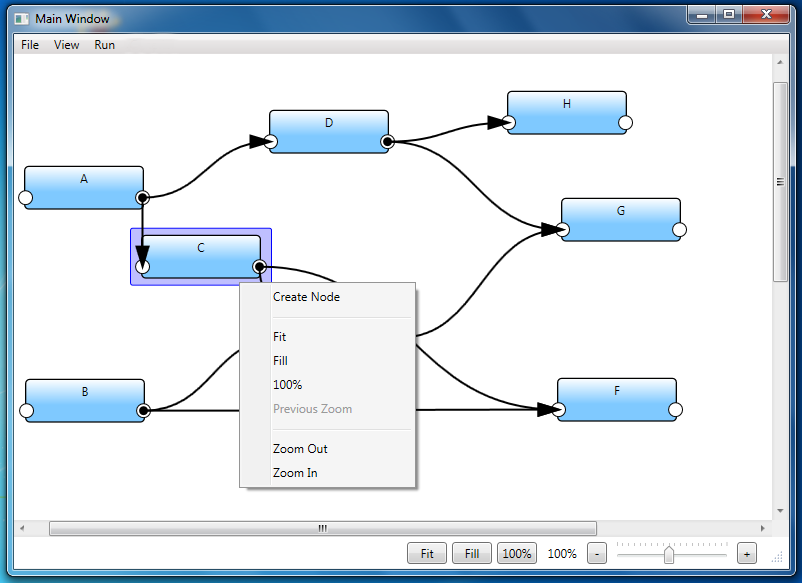
\includegraphics[width=0.85\textwidth]{app-sample-graph.png}
  }
  \caption{Вызов контекстного меню}
  \label{fig:app-sample-graph}
\end{figure}

\begin{figure}[h!]
  \centering
  {
    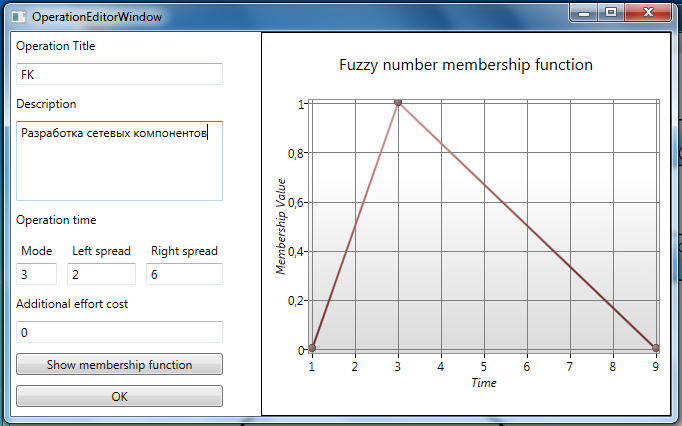
\includegraphics[width=0.9\textwidth]{app-edit-window.png}
  }
  \caption{Окно редактирования характеристик операции}
  \label{fig:app-edit-window}
\end{figure}

Удалить существующую вершину или дугу можно, щёлкнув по всплывающей кнопке в виде ножниц, которя появляется, если задержать над дугой/вершиной курсор мыши (рисунок~\ref{fig:app-scissors-button}). 
\begin{figure}[h!]
  \centering
  {
    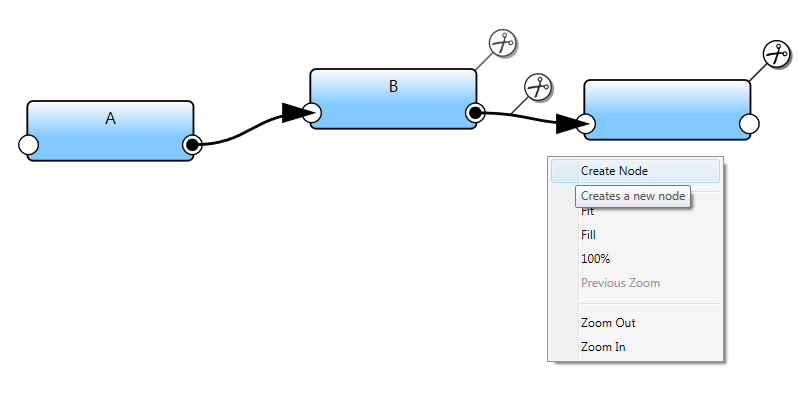
\includegraphics[width=0.8\textwidth]{app-scissors-button.png}
  }
  \caption{Всплывающие кнопки удаления элементов графа}
  \label{fig:app-scissors-button}
\end{figure}

Пункт меню <<Run>> (Запустить) показывает окно, в котором можно выбрать используемое в процессе анализа значение $\lambda$ из списка предопределённых опций (середина отрезка, центр тяжести, оптимум сохранения информации). После выбора пользователем значения $\lambda$, приложение запускает процедуру анализа. По её окончании показывается диалог, позволяющий выбрать место сохранения отчёта в формате Microsoft Excel.

Для выхода из приложения необходимо выбрать пункт меню <<File~--- Exit>> (Файл~--- Выйти) или нажать на стандартную кнопку закрытия окна в правом верхнем углу.

\subsubsection*{Функциональные возможности программы}
Программа имеет следующие функциональные возможности:
\begin{itemize}
  \item создание модели проекта в виде вершинного графа в ручном режиме или импорт существующей модели из XML-файла;
  \item поддержка модели проекта в согласованном состоянии~--- проверка отсутствия циклов в графе и наличие только одной компоненты связности;
  \item редактирование временных оценок выполнения операций, выраженных в~виде треугольных чисел, c~помощью изменения параметров нечёткго числа;
  \item графическое представление функций принадлежности для~временных оценок;
  \item автоматическое преобразование вершинного графа в~стрелочный;
  \item выбор пользователем используемых при~расчётах значений параметров $\lambda$ преобразования $L$, соответствующих середине $\alpha$-сечения, проекции центра тяжести или оптимальному в смысле сохранения экспертной информации значению;
  \item реализация механизма расчёта критического пути на~основе $\alpha$-уровневых и~двухточечных вычислений;
  \item экспорт отчёта о~решении задачи в~формат Microsoft Excel с~формированием графиков для модифицированных нечётких оценок, общего времени выполнения проекта и~построением преобразованного стрелочного графа c~выделением критических операций.
\end{itemize}

\subsubsection*{Реализация}

\textit{Структура данных}

Входными данными приложения является либо результаты пользовательского ввода, либо документ с описанием структуры проекта и временных оценок. Поскольку моделью проекта является разреженный вершинный граф, то для его хранения в памяти и на диске выбрана структура в виде списков смежности, в которой для каждой вершины указывается список идентификаторов связанных с ней вершин, а также кортеж из трёх действительных чисел, формирующих нечёткую оценку веса вершины. На диске модель проекта хранится в формате XML, что позволяет легко редактировать её.

Выходные данные агрегируются в формат Microsoft Excel и состоят из следующих частей:
\begin{itemize}
  \item две таблицы, соответствующие значениям $\alpha=0$ и $\alpha=1$ и содержащие рассчитанные для каждой операции проекта наиболее ранние и наиболее поздние сроки наступления её начального и конечного событий, а также полные резервы времени. Операции, принадлежащие критическому пути, выделены цветом;
  \item изображение полученного в результате преобразования стрелочного графа с нанесённым на него критическим путём;
  \item графики функций принадлежности для модифицированных нечётких продолжительностей операций.
\end{itemize}

\textit{Логическая структура программы}

Программа состоит из нескольких модулей, организованных в соответствие с шаблоном <<модель--представление--модель представления>>~\cite{NetworkView_CodeProject}. Схема взаимодействия между модулями программы показана на рисунке~\ref{fig:app-architecture}.
\begin{figure}[t!]
  \centering
  {
    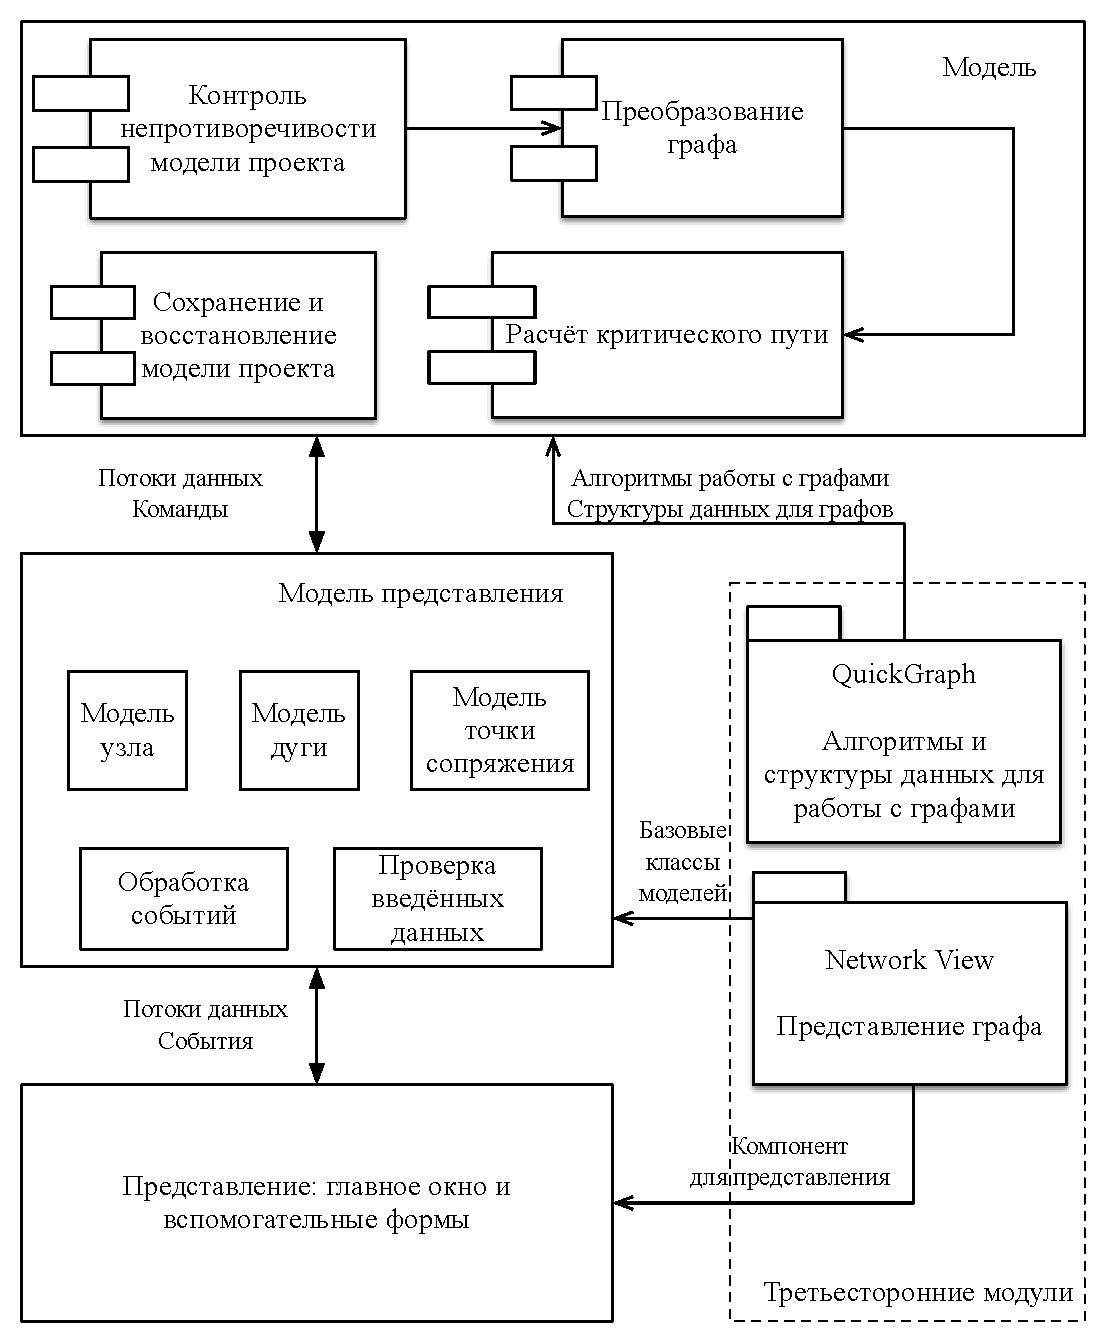
\includegraphics[width=0.7\textwidth]{app-architecture}
  }
  \caption{Взаимодействие между модулями приложения}
  \label{fig:app-architecture}
\end{figure}

Как видно из рисунка~\ref{fig:app-architecture}, в~программе были использованы третьесторонние компоненты, позволившие сократить общее время разработки и упростить тестирование~--- библиотека для~работы с~графами QuickGraph~\cite{QuickGraph_Codeplex, QuickGraph_CodeProject} и~компонент для~визуального представления и~редактирования графа NetworkView~\cite{NetworkView_CodeProject}.

В программном модуле реализован алгоритм автоматического преобразования вершинного графа в стрелочный, описанный на стр.~\pageref{ConversionAlgo}. Автоматический контроль согласованности выполняется с~помощью алгоритма поиска в~глубину при~добавлении каждой новой вершины.

\subsubsection*{Тестирование приложения}

Результаты тестирования приложения приведены в таблице~\ref{t:app-testing}.

\begin{center}
\begin{longtable}[h!]{|p{6.45cm}|p{0.55\linewidth}|}
\caption{Результаты тестирования приложения} \label{t:app-testing}\\
    \hline
      \textbf{Тест} & \textbf{Результат теста} \tabularnewline \hline
	\endfirsthead
	\caption*{Продолжение таблицы~\ref{t:app-testing}} \\
    \hline
	  \textbf{Тест} & \textbf{Результат теста} \tabularnewline \hline
	\endhead
	\hline
		Проверка доступности пунктов меню и кнопок на форме приложения & Доступны пункты меню \\ \hline
        Выбор пункта меню <<File~--- New Project>> (Файл~--- Новый проект) & Создаётся новый проект и показывается пустая рабочая область окна \\ \hline
		Выбор пункта меню <<File~--- Open existing Project>> (Файл~--- Открыть существующий проект) & Показывается диалог выбора файла с расширением *.csbgproj. Выбор файла и нажатие на кнопку <<Открыть>> приводит к загрузке проекта и его отображению на экране \\ \hline
        Выбор пункта меню <<File~--- Save Current Project>> (Файл~--- Сохранить текущий проект) & Показывается диалог сохранения файла с расширением *.csbgproj. По нажании на кнопку <<Сохранить>> создаётся файл проекта с указанным именем в указанной папке \\ \hline
		Вызов контекстного меню и выбор опции <<Create Node>> (Создать узел) & Создаётся новая вершина графа и открывается окно редактирования параметров операции. При не полностью введённых данных программа выдаёт предупреждение. При нажатии на кнопку <<Show membership function>> (Показать функцию принадлежности) строится график функции принадлежности треугольного числа с указанными параметрами. Кнопка <<OK>> позволяет закончить редактирование и продолжить работу с проектом \\ \hline
		Выделение вершины графа и выбор пункта меню <<View>> (Просмотр) & Открывается окно редактирования параметров операции\\ \hline
		Нажатие левой кнопки мыши на точке сопряжения, перетаскивание курсора мыши при зажатой левой кнопке и отпускание мыши на целевой вершине & Создаётся дуга графа между двумя вершинами \\ \hline
		Создание дуги из одной вершины в другую при наличии обратной дуги & Приложение выдаёт предупреждение о невозможности операции ввиду нарушения свойства ацикличности и не создаёт дугу \\ \hline
		Нажатие кнопки с изображением ножниц, связанной с дугой & Удаление дуги графа \\ \hline
		Нажатие кнопки с изображением ножниц, связанной с вершиной & Удаление вершины графа и всех связанных с ней дуг~--- входящих и исходящих \\ \hline
		Выбор пункта меню <<Run>> & Проверка числа компонент связности графа~--- если их больше одной, то приложение выдаёт предупреждение о невозможности запуска анализа. Иначе предлагается выбор значения параметра преобразования $L$. После выбора пользователем предпочитаемого значения параметра запускается анализ проекта, по окончании которого приложение выводит диалог сохранения отчёта в формате Microsoft Excel \\ \hline
		Нажатие стандартной кнопки <<Закрыть окно>> или выбор пункта меню <<File~--- Exit>> (Файл~--- Выход) & Завершение работы приложения \\
    \hline
\end{longtable}
\end{center}